\chapter{Experimental results (WIP)} \label{ch:ch5}

In the previous chapters, we described the reinforcement learning control system we designed, together with an analysis of the solutions we proposed for the problems we faced during the development process.
Indeed, this process has not been free from difficulties, both of implementation level and parameter optimisation.
After completing the design of this architecture, our second goal was to look for an algorithm that could better adapt to a real context, exceeding the limits set by DDPG.
The ideal would have been to find an algorithm altogether parameter agnostic: an enabling feature to achieve excellent performance regardless of the specific configuration.
During our research we came across the SAC algorithm and, after a careful analysis of the paper and having understood the considerations made by the authors about SAC real-world applications, we thought it might be the right choice to get better performance than the DDPG experiments.
For this reason, this chapter aims to present a detailed comparison of the experiments carried out on both algorithms.

The first section of this chapter focuses on the experimental methodology.
It will be an opportunity to describe the hardware of the development machine we used for the experiments and present in a more schematic and precise way the OpenAI Gym environments on which we will apply the algorithms.
We speak in the plural, because we have decided to report both the experiments performed on \textit{Pendulum-v0} environment, and those carried out with Anki Cozmo in the real world using the architecture we built.
This part will also contain a brief analysis of how reinforcement learning experiments are assessed to date.
For this segment, we took inspiration by \cite{henderson2018deep}, an exciting publication where the authors investigated reproducibility challenges, proper experimental techniques, and reporting procedures of modern deep reinforcement learning to draw up guidelines from which to start in order to obtain better reports, not so much from the result perspective, but from how they are reported.

The second and third sections of this chapter will, therefore, be devoted respectively to the two types of environments used.
We have shown all the useful graphs in order to analyse and to comment on the obtained results.

\section{Experimental Methodology}

This pre-trial section is essential to better understand the tasks we tried to get the reinforcement learning algorithms to solve and what approach we used to evaluate experiments results.

\subsection{Hardware and Software details}

In order to carry out the experiments contained in this chapter we have made use of a personal computer.

\subsection{Pendulum-v0 Environment}

The inverted pendulum swingup problem is a classic problem in the control literature. In this version of the problem, the pendulum starts in a random position, and the goal is to swing it up so it stays upright.
	%\begin{figure}[ht!]
	%	\centering
	%	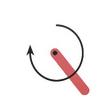
\includegraphics[height=0.2\paperwidth]{img/pendulum.png}
	%	\caption{Frame of Pendulum-v0 environment}
	%	\label{fig:pendulum}
	%\end{figure}
	\paragraph{Observation}
	Type: Box(3)
	\begin{table}[!h]
		\centering
		% \caption{MountainCarContinuous-v0 Observation}
		\label{mountain_observation}
		\begin{tabular}{@{}lllll@{}}
			\toprule
			Index	& Observation		& Min 		& Max 		\\ \midrule
			0			& cos($\theta$)	 	&  $-1.0$	& $+1.0$ 	\\
			1			& sin($\theta$)	 	&  $-1.0$		& $+1.0$ \\
			2			& $\dot{\theta}$	 	&  $-8.0$		& $+8.0$ \\
			\bottomrule
		\end{tabular}
	\end{table}
	\paragraph{Actions}
	Type: Box(1)
	\begin{table}[!h]
		\centering
		% \caption{MountainCarContinuous-v0 Actions }
		\label{mountain_action}
		\begin{tabular}{@{}lllll@{}}
			\toprule
			Index	& Action	& Min 		& Max 		\\ \midrule
			0			& Joint effort &  $-2.0$	& $+2.0$ 	\\
			\bottomrule
		\end{tabular}
	\end{table}
	
	\paragraph{Reward}
	The reward for each timestep $t$ is given by \[r_t = -(\theta_t^2 + 0.1 \dot{\theta}^2 + 0.001 a_t^2)\]
	where theta is normalized between $-\pi$ and $\pi$. Therefore, the lowest cost is $-(\pi^2 + 0.1*8^2 + 0.001*2^2) = -16.2736044$, and the highest cost is $0$. In essence, the goal is to remain at zero angle (vertical), with the least rotational velocity, and the least effort.
	
	\paragraph{Starting State}
	Random angle from $-\pi$ to $\pi$, and random velocity between $-1$ and $1$
	\paragraph{Episode Termination}
	There is no specified termination. Adding a maximum number of steps might be a good idea. In this case 200.
	\paragraph{Solved Requirements}
	It is an unsolved environment, which means it does not have a specified reward threshold at which it is considered solved.
	


\subsection{CozmoEnv-v0 Environment}

\section{Pendulum-v0 Experiments}

\subsection{Comparative Analysis}

\subsection{Results}

\section{CozmoEnv-v0 Experiments}

\subsection{Comparative Analysis}

\subsection{Results}



\todomacaluso{
	\begin{itemize}
		\item Introduction: arguments of the chapter and overview of final results
		\item Experimental Methodology
		      \begin{itemize}
			      \item Preliminaries: experiments with Pendulum-v0
			      \item Real Life experiments with Cozmo
			      \item Hyper-Parameters discussion and motivation
			      \item Algorithms applied and modifications with pseudo-code
		      \end{itemize}
		\item Experiments with Pendulum-v0
		      \begin{itemize}
			      \item Comparative analysis between results obtained with DDPG and SAC
			      \item Results
		      \end{itemize}
		\item Experiments with Cozmo
		      \begin{itemize}
			      \item Comparative analysis between results obtained with DDPG and SAC
			      \item Results
		      \end{itemize}
	\end{itemize}
}
